\documentclass[12pt,a4]{ctexart}
\usepackage{natbib}
\usepackage{url}
\usepackage{stmaryrd}
\usepackage{mathrsfs}
\usepackage{amsmath}
\usepackage{graphicx}
\usepackage{parskip}
\usepackage{fancyhdr}
% \usepackage{underscore} % 下划线
\usepackage{commath}%定义d
\usepackage{geometry}
\usepackage{bm}
\usepackage{siunitx}
\usepackage{float}
% \usepackage[skip=-5pt]{subcaption}
% \usepackage{subfig}
\usepackage{subfigure}  %插入多图时用子图显示的宏包
\usepackage{titlesec}
\usepackage{caption}
\usepackage{paralist}
\usepackage{multirow}
\usepackage{booktabs} % To thicken table lines
\usepackage{diagbox}
\usepackage{authblk}
\usepackage{indentfirst}
\usepackage{amsthm}
\usepackage{fontspec}
\usepackage{color}
%\usepackage{txfonts} %设置字体为times new roman
\usepackage{lettrine}
\usepackage{nameref}
%\usepackage[nottoc]{tocbibind}
\usepackage{amssymb}%font
\usepackage{lipsum}%make test words
\usepackage{picinpar}%words around the picture
\usepackage[all]{xy}%draw arrow
\usepackage{asymptote}%draw picture
\usepackage[perpage]{footmisc}%脚注每页清零
\usepackage{esint}
\renewcommand{\proofname}{\indent \sf \bfseries{证明}}
\pagestyle{fancy}
\fancyhf{}
\renewcommand{\headrulewidth}{0pt}
\fancyfoot[C]{\thepage}

\catcode`\。=\active
\catcode`\,=\active
\catcode`\;=\active
\catcode`\:=\active
\newcommand{。}{.}
\newcommand{,}{,}
\newcommand{;}{;}
\newcommand{:}{:}

\geometry{bottom=3cm,left=3cm,right=3cm,a4paper, top=2.5cm}
% \footskip = 60pt

% \setmainfont{TimesNewRomanPSMT}
% \setsansfont{Helvetica-Light}
\setCJKmainfont[ItalicFont=STKaitiSC-Regular,BoldFont=SimSong-Bold]{SimSong-Regular}
\setCJKsansfont[BoldFont=STHeitiSC-Medium]{STHeitiSC-Light}


%\setmainfont{Times New Roman}

\ctexset{today=old}%日期类型设置

% ======================================
% = Color de la Universidad de Sevilla =
% ======================================
\usepackage{tikz}
\definecolor{PKUred}{cmyk}{0,1,1,0.45}

%超链接设置
\usepackage[breaklinks,colorlinks,linkcolor=PKUred,citecolor=PKUred,pagebackref,urlcolor=PKUred]{hyperref}
\usepackage{cleveref}
\newcommand{\crefpairconjunction}{ 和 }
% \newcommand{\crefmiddleconjunction}{ 和 } 
\newcommand{\creflastconjunction}{ 和 }

\newcommand{\hsp}{\hspace{20pt}}
\newcommand{\nhsp}{\hspace{-30pt}}
% \titleformat{\section}{\Large\bfseries}{%\arabic{section}
% \hspace{-22pt}\textcolor{PKUred}{\vrule width 2pt}\hsp}{0pt}{}


% \titleformat{\subsection}
% {\normalfont\large\bfseries}{}{0em}{}

\renewcommand*\footnoterule{%
   \vspace*{-3pt}%
   {\color{PKUred}\hrule width 2in height 0.4pt}%
   \vspace*{2.6pt}%
}


%% Color the bullets of the itemize environment and make the symbol of the third
%% level a diamond instead of an asterisk.
%h\renewcommand*\textbullet{\dag}
\renewcommand*\labelitemi{\color{PKUred}\textbullet}
\renewcommand*\labelitemii{\color{PKUred}--}
\renewcommand*\labelitemiii{\color{PKUred}$\diamond$}
\renewcommand*\labelitemiv{\color{PKUred}\textperiodcentered}



%%% Equation and float numbering
\numberwithin{equation}{section}		% Equationnumbering: section.eq#
\numberwithin{figure}{section}			% Figurenumbering: section.fig#
\numberwithin{table}{section}				% Tablenumbering: section.tab#


%代码设置
\usepackage{listings}
\usepackage{accsupp}
\usepackage{fontspec} % 定制字体
\newfontfamily\menlo{Menlo-Regular}
\usepackage{xcolor} % 定制颜色
\definecolor{mygreen}{rgb}{0,0.6,0}
\definecolor{mygray}{rgb}{0.5,0.5,0.5}
\definecolor{mymauve}{rgb}{0.58,0,0.82}
\lstset{
   numbers=left,
   numberstyle=\footnotesize\menlo,
   basicstyle=\footnotesize\menlo,
   backgroundcolor=\color{white},      % choose the background color
   columns=fullflexible,
   tabsize=4,
   breaklines=true,               % automatic line breaking only at whitespace
   captionpos=b,                  % sets the caption-position to bottom
   commentstyle=\color{mygreen},  % comment style
   escapeinside={\%*}{*)},        % if you want to add LaTeX within your code
   keywordstyle=\color{blue},     % keyword style
   stringstyle=\color{mymauve}\ttfamily,  % string literal style
   frame=lrtb,
   rulesepcolor=\color{red!20!green!20!blue!20},
   % identifierstyle=\color{red},
   % language=c++,
   xleftmargin=4em,xrightmargin=2em, aboveskip=1em,
   % framexleftmargin=2em,
   numbers=left
}

%脚注
\renewcommand\thefootnote{\fnsymbol{footnote}}

%定义常数i、e、积分符号d
\newcommand\mi{\mathrm{i}}
\newcommand\me{\mathrm{e}}

%%% Maketitle metadata
\newcommand{\horrule}[1]{\rule{\linewidth}{#1}} 	% Horizontal rule
\newcommand{\tabincell}[2]{\begin{tabular}{@{}#1@{}}#2\end{tabular}}


\setcounter{secnumdepth}{2}
\usepackage{bm}
\usepackage{autobreak}
\usepackage{amsmath}
\setlength{\parindent}{2em}
\graphicspath{{../}}


%pdf文件设置
\hypersetup{
	pdfauthor={袁磊祺},
	pdftitle={湍流2}
}

\title{
	\vspace{-1in} 	
	\usefont{OT1}{bch}{b}{n}
	\normalfont \normalsize \textsc{\LARGE Peking University}\\[1cm] % Name of your university/college \\ [25pt]
	\horrule{0.5pt} \\[0.5cm]
	\huge \bfseries{湍流2} \\
	\horrule{2pt} \\[0.5cm]
}
\author{
	\normalfont 								\normalsize
	College of Engineering \quad 2001111690  \quad 袁磊祺\\	\normalsize
	\today
}
\date{}

\begin{document}

%%%%%%%%%%%%%%%%%%%%%%%%%%%%%%%%%%%%%%%%%%%%%%
\captionsetup[figure]{name={图},labelsep=period}
\captionsetup[table]{name={表},labelsep=period}
\renewcommand\contentsname{目录}
\renewcommand\listfigurename{插图目录}
\renewcommand\listtablename{表格目录}
\renewcommand\refname{参考文献}
\renewcommand\indexname{索引}
\renewcommand\figurename{图}
\renewcommand\tablename{表}
\renewcommand\abstractname{摘\quad 要}
\renewcommand\partname{部分}
\renewcommand\appendixname{附录}
\def\equationautorefname{式}%
\def\footnoteautorefname{脚注}%
\def\itemautorefname{项}%
\def\figureautorefname{图}%
\def\tableautorefname{表}%
\def\partautorefname{篇}%
\def\appendixautorefname{附录}%
\def\chapterautorefname{章}%
\def\sectionautorefname{节}%
\def\subsectionautorefname{小小节}%
\def\subsubsectionautorefname{subsubsection}%
\def\paragraphautorefname{段落}%
\def\subparagraphautorefname{子段落}%
\def\FancyVerbLineautorefname{行}%
\def\theoremautorefname{定理}%
\crefname{figure}{图}{图}
\crefname{equation}{式}{式}
\crefname{table}{表}{表}
%%%%%%%%%%%%%%%%%%%%%%%%%%%%%%%%%%%%%%%%%%%

\maketitle

2021 年 11 月 3 日前交电子版

代码等作业内容可在 \texttt{\href{https://github.com/circlelq/Turbulence}{https://github.com/circlelq/Turbulence}} 查看。

\section{1}

推导两个独立随机变量乘积的概率密度表达式。

\textsf{\hspace{-2em}\sf  \textbf{解:}}

Given two continuous random variables, x and y, along with their joint probability density, $P(x,y)$, we wish to find the probability density of a new random variable, $s$, that is some function of the original random variables, $s = f (x, y)$. The formal solution can be written in terms of a Dirac delta function.\cite{Swendsen}
\begin{equation}
	P(s)=\int_{-\infty}^{\infty} \int_{-\infty}^{\infty} P(x, y) \delta(s-f(x, y)) \dif x \dif y.
	\label{eq:1Dirac}
\end{equation}
As was the case for the corresponding discrete random variables, the probability density of $s$ is automatically normalized.
\begin{equation}
	\begin{aligned}
		\int_{-\infty}^{\infty} P(s) \dif s & =\int_{-\infty}^{\infty} \int_{-\infty}^{\infty} \int_{-\infty}^{\infty} P(x, y) \delta(s-f(x, y)) \dif s \dif x \dif y \\
		                                    & =\int_{-\infty}^{\infty} \int_{-\infty}^{\infty} P(x, y) \dif x \dif y=1.
	\end{aligned}
\end{equation}
The last equality is due to the normalization of $P(x, y)$.

此题中$f (x, y) = x y $, 又由于两个变量是独立的,所以$P(x,y) = P(x) P(y)$.代入\cref{eq:1Dirac}可得
\begin{equation}
	\begin{aligned}
		P(s) & =\int_{-\infty}^{\infty} \int_{-\infty}^{\infty} P(x, y) \delta(s-f(x, y)) \dif x \dif y                        \\
		     & =\int_{-\infty}^{\infty} \int_{-\infty}^{\infty} P_X(x) P_Y(y) \delta(s-xy) \dif x \dif y                       \\
		     & =\int_{-\infty}^{\infty} \dif x P_X(x) \frac{1}{\abs{x}} \int_{-\infty}^{\infty}   P_Y(y) \delta(s/x-y)  \dif y \\
		     & =\int_{-\infty}^{\infty}  P_X(x) \frac{1}{\abs{x}} P_Y(s/x) \dif x                                              \\
	\end{aligned}
\end{equation}

\section{2}

证明: 两个独立的高斯分布随机变量之比的概率密度为柯西分布。

设两个独立的高斯分布随机变量为
\begin{equation}
	P(x) = \frac{1}{\sqrt{2\pi}} \me^{-\frac{x^2}{2}},
\end{equation}
\begin{equation}
	P(y) = \frac{1}{\sqrt{2\pi}} \me^{-\frac{y^2}{2}}.
\end{equation}
新的变量$f(x,y) = y / x$,根据\cref{eq:1Dirac}可得
\begin{equation}
	\begin{aligned}
		P(s) & =\int_{-\infty}^{\infty} \int_{-\infty}^{\infty} P(x, y) \delta(s-f(x, y)) \dif x \dif y              \\
		     & =\int_{-\infty}^{\infty} \int_{-\infty}^{\infty} P_X(x) P_Y(y) \delta(s-y/x) \dif x \dif y            \\
		     & =\int_{-\infty}^{\infty} \dif x \abs{x} P_X(x)  \int_{-\infty}^{\infty}   P_Y(y) \delta(sx-y)  \dif y \\
		     & =\int_{-\infty}^{\infty} \abs{x} P_X(x) P_Y(sx) \dif x                                                \\
		     & = \frac{1}{2\pi} \int_{-\infty}^{\infty} \abs{x} \me^{-\frac{x^2}{2}} \me^{-\frac{s^2x^2}{2}} \dif x  \\
		     & = \frac{1}{\pi (s^2+1)}.
	\end{aligned}
\end{equation}\qed



\section{3}

对于概率密度 $p(x)$, 定义 $H=-\int p \ln p \dif x$ 为此概率分布的熵。那么, 当给定 数学期望和方差时, 求熵最大的概率密度函数。

\textsf{\hspace{-2em}\sf  \textbf{解:}}

设数学期望和方差为
\begin{equation}
	\mu = \int x p(x) \dif x, \quad \sigma = \int (x-\mu)^2 p(x) \dif x.
	\label{eq:3exp}
\end{equation}
这里省略了上下限$+\infty,-\infty$,由归一化有
\begin{equation}
	\int p(x) \dif x = 1,
	\label{eq:3guiyi}
\end{equation}
拉格朗日乘子式
\begin{equation}
	\begin{aligned}
		L(p) = & - \int p \ln p \dif x + \lambda_0 \left(1- \int p \dif x\right)                                            \\
		       & + \lambda_1 \left( \mu - \int x p \dif x\right) + \lambda_2 \left(\sigma - \int (x-\mu)^2 p \dif x\right).
	\end{aligned}
\end{equation}
对$L(p)$求$p$的变分,得到下式
\begin{equation}
	\delta L(p)  = - \int \left( 1 + \ln p + \lambda_0 + \lambda_1 x - \lambda_2 (x-\mu)^2 \right) \delta p \dif x = 0.
\end{equation}
所以
\begin{equation}
	1 + \ln p + \lambda_0 + \lambda_1 x - \lambda_2 (x-\mu)^2 = 0,
\end{equation}
\begin{equation}
	p = \me^{-1-\lambda_0 - \lambda_1 x + \lambda_2 (x-\mu)^2}.
\end{equation}
根据\cref{eq:3exp,eq:3guiyi}可求出系数,最终得
\begin{equation}
	p(x)=\frac{1}{\sqrt{2 \pi} \sigma} \exp \left(-\frac{(x-\mu)^{2}}{2 \sigma^{2}}\right).
\end{equation}


\section{4}

设 $U, V$ 是两个在 $(0,1]$ 上均匀分布的独立随机变量, 若
\begin{equation}
	X=\sqrt{-2 \ln U} \cos (2 \pi V),\quad Y=\sqrt{-2 \ln U} \sin (2 \pi V),
\end{equation}
试证: $X$ 与 $Y$ 是两个独立的标准高斯分布的随机变量。

根据\cite[P91]{THU-stat}中的定理2.5.2有
\begin{equation}
	f_{(X,Y)}(x,y) =f_{(U,V)} (u(x,y),v(x,y)) \abs{J}
\end{equation}
其中$J$是雅可比矩阵
\begin{equation}
	J = \frac{\partial (u,v)}{\partial (x,y)}.
\end{equation}
通过{Matlab}代码
\begin{lstlisting}[language=matlab]
syms x y
a = [x y];
f = [exp(-1/2*(x^2+y^2)) atan(y/x)/2/pi];
ja = jacobian(f, a)
det(ja)	
\end{lstlisting}
可以求得
\begin{equation}
	\abs{J} = \frac{{\mathrm{e}}^{-\frac{x^2 }{2}-\frac{y^2 }{2}} }{2\,\pi },
\end{equation}
由于概率分布为正,所以上式已经取了一个绝对值。由均匀分布有
\begin{equation}
	f_{(U,V)} (u(x,y),v(x,y)) = 1,
\end{equation}
所以
\begin{equation}
	f_{(X,Y)}(x,y) = \frac{{\mathrm{e}}^{-\frac{x^2 }{2}-\frac{y^2 }{2}} }{2\,\pi }.
\end{equation}
由此可见$X$ 与 $Y$ 是两个独立的标准高斯分布的随机变量。\qed


\section{5}

对于 $[0,1]$ 上的分布, 证明其各阶矩构成一个完全单调序列。

$k$阶矩
\begin{equation}
	\sigma_n \equiv \int^{+\infty}_{-\infty} x^n p(x) \dif x,\quad n \geqslant 0, \quad n \in \mathbb{Z}^+.
\end{equation}

对$\forall \{ \xi_i \}$,
\begin{equation}
	\begin{aligned}
		\sum_{i,j} \sigma_{i+j}
		\xi_i \xi_j & = \sum_{i,j} \int^{+\infty}_{-\infty} x^{i+j} \xi_i \xi_j p(x) \dif x         \\
		            & = \int^{+\infty}_{-\infty} \sum_{i,j} x^{i} \xi_i x^j \xi_j p(x) \dif x       \\
		            & = \int^{+\infty}_{-\infty}  \left( \sum_{i} x^{i} \xi_i \right)^2 p(x) \dif x \\
		            & \geqslant 0.
	\end{aligned}
\end{equation}
其中$i,j\in \mathbb{Z}^+$.\qed


\section{6}

对于如下稳定分布的特征函数 $\varphi(s)= \exp\left(-|s|^{1 / 2}\right)$, 画出其概率密度函数, 并 验证概率密度函数的尾部渐近于幂次律, 求出幂指数(的近似值)。

\textsf{\hspace{-2em}\sf  \textbf{解:}}

由于
\begin{equation}
	\int^{+\infty}_0 \exp\left(-|s|^{1 / 2}\right) \dif s = 2,
\end{equation}
所以特征函数是绝对可积的,则对特征函数做逆变换有\cite[P190]{wangzikun}
\begin{equation}
	p(x)=F^{\prime}(x)=\frac{1}{2 \pi} \int_{\mathbb{R}} \me^{-\mi t x} \varphi(t) \dif t = \frac{1}{2 \pi} \int_{\mathbb{R}} \me^{-\mi t x} \exp\left(-|t|^{1 / 2}\right) \dif t.
\end{equation}
如\cref{fig:6pdf} 所示,尾部确实近似为幂次律,幂指数近似为$-1.34$.
\begin{figure}[htp]
	\centering
	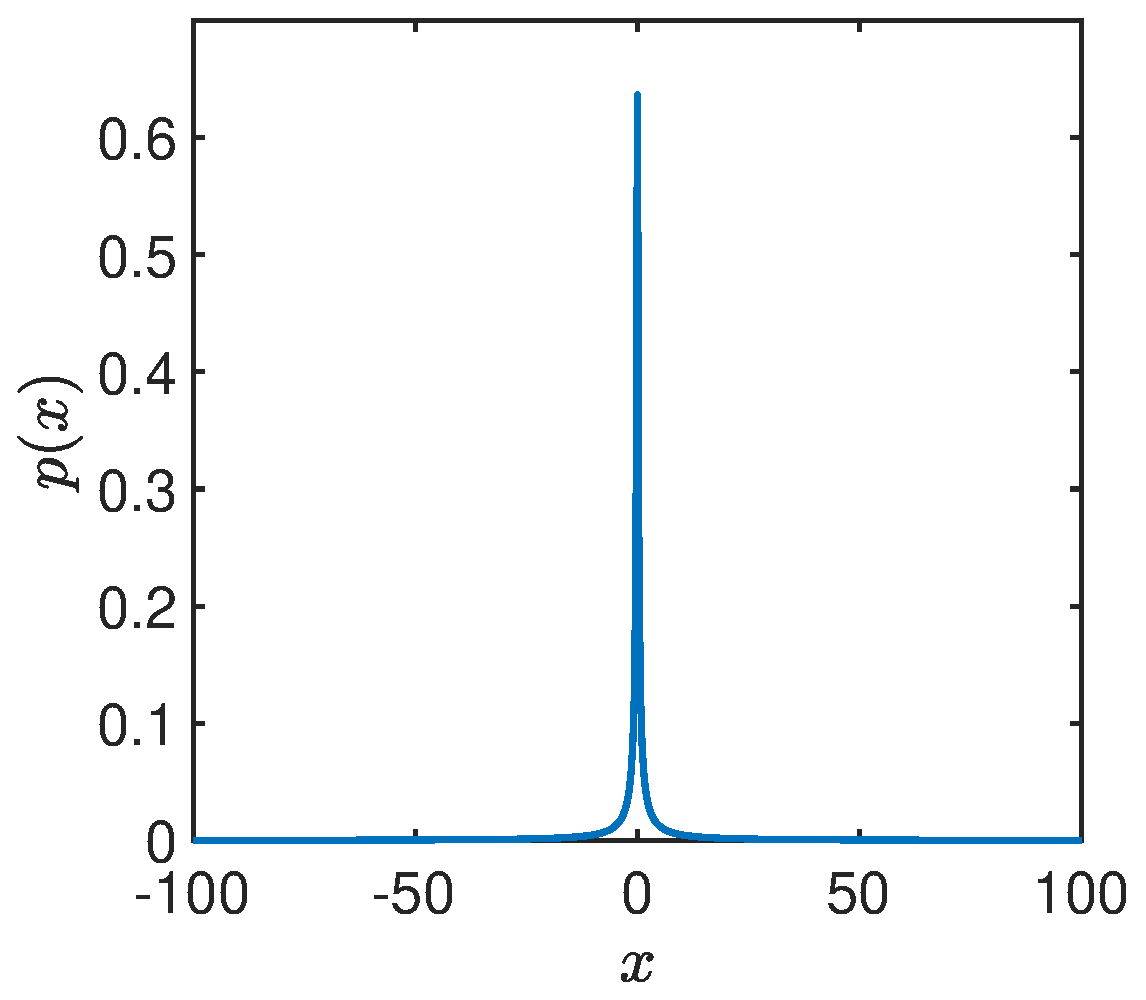
\includegraphics[scale=0.33]{6pdf.eps}
	\hspace{0.5in}
	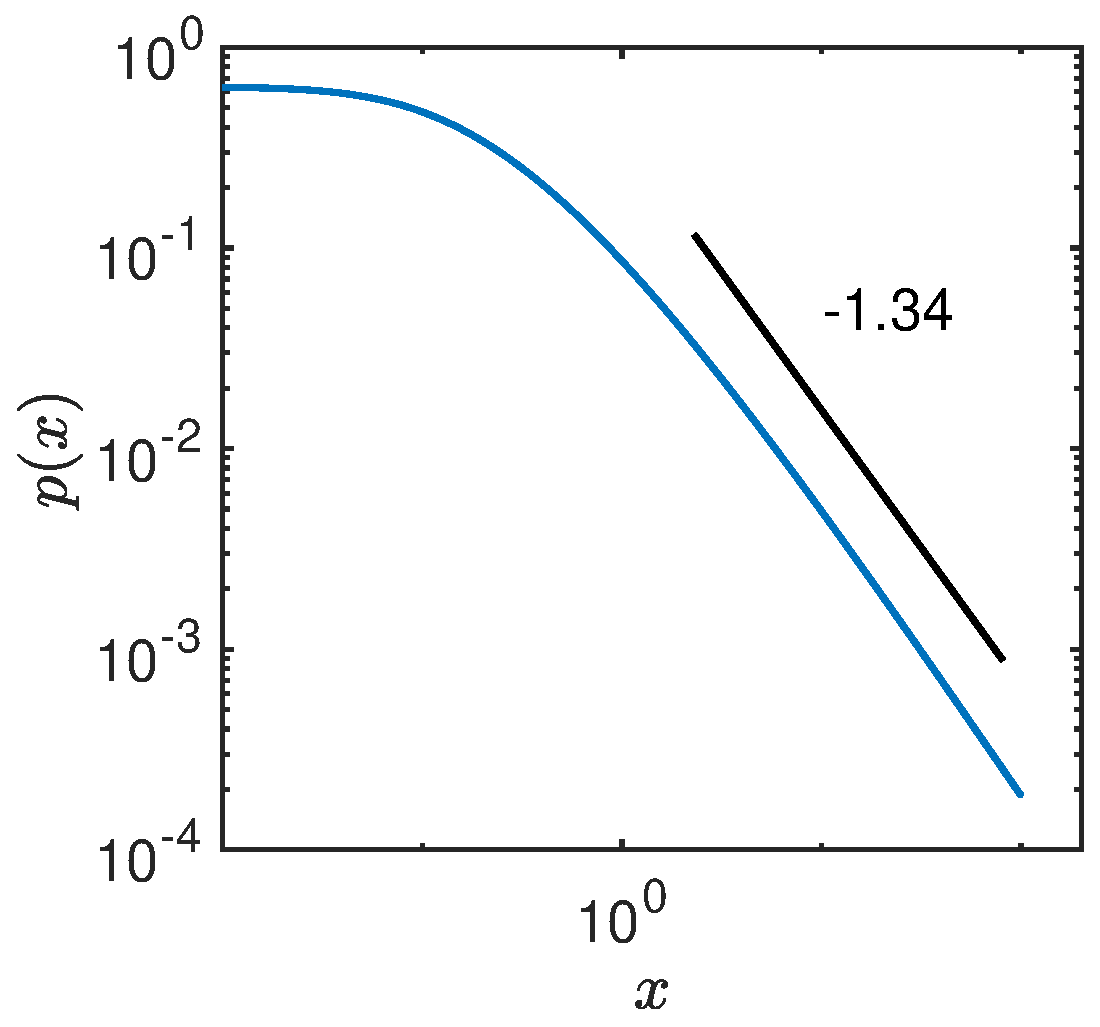
\includegraphics[scale=0.33]{6log.eps}
	\caption{概率密度函数及尾部双对数坐标图.}
	\label{fig:6pdf}
\end{figure}


\section{7}


设 $X(t)$ 是一个零均值的平稳随机过程, 其自相关函数为 $R(\tau)=\me^{-a|\tau|},\ a>0$。 定义
\begin{equation}
	Y(t)=\frac{1}{t} \int_{0}^{t} X(\tau) \dif \tau.
\end{equation}
求 $Y(t)$ 的自相关函数。

\textsf{\hspace{-2em}\sf  \textbf{解:}}

\begin{equation}
	\begin{aligned}
		R_Y(\Delta t) & = \left\langle Y(t_1)Y(t_2)\right\rangle                                                                                          \\
		              & = \left\langle \frac{1}{t_1} \int_{0}^{t_1} X(\tau_1) \dif \tau_1 \frac{1}{t_2} \int_{0}^{t_2} X(\tau_2) \dif \tau_2\right\rangle \\
		              & = \left\langle \frac{1}{t_1 t_2} \int_{0}^{t_1} \int_{0}^{t_2} X(\tau_1)   X(\tau_2) \dif \tau_1 \dif \tau_2\right\rangle         \\
		              & = \frac{1}{t_1 t_2} \int_{0}^{t_1} \int_{0}^{t_2}\left\langle  X(\tau_1)   X(\tau_2) \right\rangle \dif \tau_1 \dif \tau_2        \\
		              & = \frac{1}{t_1 t_2} \int_{0}^{t_1} \int_{0}^{t_2} \me^{-a|\tau_1-\tau_2|} \dif \tau_1 \dif \tau_2,                                \\
	\end{aligned}
\end{equation}
不妨设$t_1 \geqslant t_2$,
\begin{equation}
	\begin{aligned}
		R_Y(\Delta t) & = \frac{1}{t_1 t_2} \int_{0}^{t_1} \int_{0}^{t_2} \me^{-a|\tau_1-\tau_2|} \dif \tau_1 \dif \tau_2,                                                                                                                                            \\
		              & = \frac{1}{t_1 t_2} \left(\int^{t_2}_0 (t_2 - \tau) \me^{-a \tau} \dif \tau +  \int^{t_1 - t_2}_0 t_2 \me^{-a \tau} \dif \tau +  \int^{t_2}_0 (t_2 - \tau) \me^{-a (\tau+t_1-t_2)} \dif \tau   \right)                                        \\
		              & = \frac{1}{t_1 t_2} \left( \dfrac{\mathrm{e}^{-at_2}}{a^2}+\dfrac{at_2-1}{a^2} + t_2\left(\dfrac{1}{a}-\dfrac{\mathrm{e}^{at_2-at_1}}{a}\right) +  \dfrac{\mathrm{e}^{-at_1}\left(\left(at_2-1\right)\mathrm{e}^{at_2}+1\right)}{a^2} \right) \\
		              & = -\dfrac{\left(\mathrm{e}^{at_2}\left(\mathrm{e}^{at_2}-\mathrm{e}^{at_1}\left(2at_2-1\right)-1\right)-\mathrm{e}^{at_1}\right)\mathrm{e}^{-a\left(t_2+t_1\right)}}{t_1 t_2 a^2}.
	\end{aligned}
\end{equation}



\section{8}


令随机过程 $Z(t)$ 为
\begin{equation}
	Z(t)=a X(t)+b Y(t)
\end{equation}
其中 $a, b$ 为常数, $X(t)$ 和 $Y(t)$ 为平稳随机过程。用 $X(t)$ 和 $Y(t)$ 的功率谱密度求 $Z(t)$ 的功率谱密度。

\textsf{\hspace{-2em}\sf  \textbf{解:}}

假设$X(t)$ 和 $Y(t)$均值为$0$,功率谱密度\cite[P101]{suiji}
\begin{equation}
	P(\omega)  =\frac{1}{2\pi} \int^{\infty}_{-\infty} R(\tau) \me^{-\mi \omega \tau} \dif \tau.
\end{equation}
\begin{equation}
	P_X(\omega)  =\frac{1}{2\pi} \int^{\infty}_{-\infty} R_X(\tau) \me^{-\mi \omega \tau} \dif \tau, \quad P_Y(\omega)  =\frac{1}{2\pi} \int^{\infty}_{-\infty} R_Y(\tau) \me^{-\mi \omega \tau} \dif \tau.
\end{equation}
\begin{equation}
	P_Z(\omega)  =\frac{1}{2\pi} \int^{\infty}_{-\infty} R_Z(\tau) \me^{-\mi \omega \tau} \dif \tau.
\end{equation}
相关函数
\begin{equation}
	\begin{aligned}
		R_Z(\tau) & = \left\langle Z(t_1) Z(t_2)\right\rangle                                                                                                                                                  \\
		          & = \left\langle (a X(t_1)+b Y(t_1)) (a X(t_2)+b Y(t_2)) \right\rangle                                                                                                                       \\
		          & = a^2 \left\langle X(t_1) X(t_2) \right\rangle + ab \left\langle X(t_1) Y(t_2) \right\rangle + ab \left\langle X(t_2) Y(t_1) \right\rangle  + b^2 \left\langle Y(t_1) Y(t_2) \right\rangle \\
		          & = a^2 \left\langle X(t_1) X(t_2) \right\rangle + b^2 \left\langle Y(t_1) Y(t_2) \right\rangle                                                                                              \\
		          & = a^2 R_X(\tau) + b^2 R_Y(\tau).                                                                                                                                                           \\
	\end{aligned}
\end{equation}
所以
\begin{equation}
	\begin{aligned}
		P_Z(\omega) & =\frac{1}{2\pi} \int^{\infty}_{-\infty} \left(a^2 R_X(\tau) + b^2 R_Y(\tau)\right) \me^{-\mi \omega \tau} \dif \tau. \\
		            & = a^2 P_X(\omega) + b^2 P_Y(\omega).
	\end{aligned}
\end{equation}



\section{9}


试确定以下随机过程是否具有遍历性:
\begin{equation}
	X(t)=A \sin \left(\omega_{0} t+\sigma B(t)+\theta \right),
\end{equation}
其中 $A,\ \omega_{0},\ \sigma$ 是正常数, $B(t)$ 是一个单位维纳过程, $\theta$ 是 $[0,2 \pi]$ 上均匀分布的随机变量, 并且与 $B(t)$ 独立。

\textsf{\hspace{-2em}\sf  \textbf{解:}}

相关函数
\begin{equation}
	\begin{aligned}
		R(\tau) & = \left\langle X(t_1) X(t_2) \right\rangle                                                                                                                                                  \\
		        & = A^2 \left\langle \sin \left(\omega_{0} t_1 + \sigma B(t_1)+\theta \right) \sin \left(\omega_{0} t_2 + \sigma B(t_2)+\theta \right) \right\rangle                                          \\
		        & = A^2 \left\langle \int_0^{2\pi} \sin \left(\omega_{0} t_1 + \sigma B(t_1)+\theta \right) \sin \left(\omega_{0} t_2 + \sigma B(t_2)+\theta \right) \dif \frac{\theta}{2\pi} \right\rangle_B \\
		        & = A^2 \left\langle  \cos \left(\omega_{0} \tau + \sigma B(\tau) \right) \right\rangle_B                                                                                                     \\
		        & = A^2 \int^{+\infty}_{-\infty}  \cos \left(\omega_{0} \tau + \sigma x \right) \frac{1}{\sqrt{2\pi}} \me^{-x^2} \dif x                                                                       \\
		        & = \frac{A^2}{\sqrt{2}} \cos(\omega_0 \tau) \me^{-\frac{\sigma^2}{4}}.
	\end{aligned}
\end{equation}
所以
\begin{equation}
	\lim_{T \to +\infty} \frac{1}{T} \int^T_0 R(\tau) \dif \tau = \lim_{T \to +\infty} \frac{1}{T} \int^T_0 \frac{A^2}{\sqrt{2}} \cos(\omega_0 \tau) \me^{-\frac{\sigma^2}{4}} \dif \tau = 0.
\end{equation}
根据各态历经定理有此随机过程具有遍历性。


\section{10}

考虑一段突扩管流包含的总动能 $K$, 在大雷诺数时它是一个随机变量。如果 管流的入口速度近似为不变的, 问 $K$ 可否近似服从对数正态分布?总耗散呢?

\textsf{\hspace{-2em}\sf  \textbf{解:}}

可以。假设初始总动能为$K_0$,经过一段时间后乘以放大系数$x_1$变成$x_1K_0$,以此类推有
\begin{equation}
	K_n = K_0 \prod_{i=1}^{n} x_i,
\end{equation}
两边取对数得
\begin{equation}
	\ln K_n = \ln K_0 +  \sum_{i=1}^{n} \ln x_i.
\end{equation}
由于$\ln x_i$是近似独立同分布的,由中心极限定理得$\ln K_n$近似符合正态分布,即$K$可近似服从对数正态分布。

根据上面一样的推导可以得总耗散可近似服从对数正态分布。或者换一个思路,假设总耗散由所有各个地方的耗散加起来,各处的耗散满足独立同分布,所以总耗散满足正态分布。


% \nocite{*}

% \newpage
\bibliographystyle{plain}
% \clearpage
\phantomsection

\addcontentsline{toc}{section}{参考文献} %向目录中添加条目,以章的名义
\bibliography{homework}

\end{document}
